\section{Ορισμός μετα-μοντέλου Συσκευής}
\label{sec:metamodel_device}

Το μετα-μοντέλο αυτό περιέχει χαρακτηριστικά που μπορεί να έχει μια συσκευή (μικροελεγκτής ή περιφερειακό) και μας χρησιμεύουν στη διαδικασία παραγωγής κώδικα. Στο \autoref{fig:metamodel_device} μπορούμε να δούμε μία απεικόνισή του.

\begin{figure}[!ht]
	\centering
	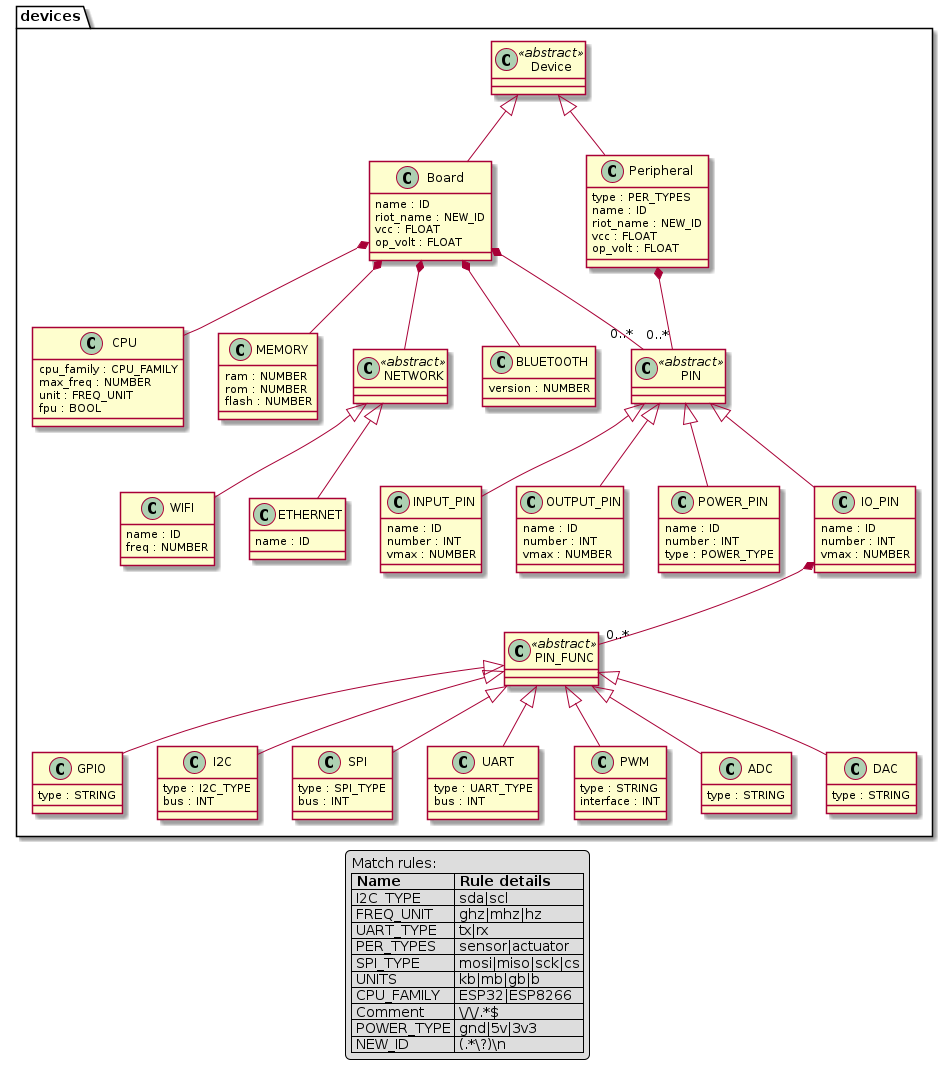
\includegraphics[height=0.8\textheight]{./images/chapter5/metamodel_device.png}
	\caption{Μετα-μοντέλο συσκευής}
	\label{fig:metamodel_device}
\end{figure}

\subsection{Device}
\label{subsec:device}

\subsubsection*{Σύνοψη}

\noindent Το στοιχείο αυτό είνια η abstract κλάση για το αν μια συσκευή είναι μικροελεγκτής ή περιφερειακό.

\subsubsection*{Ιδιότητες και Συσχετίσεις}

\noindent Δεν περιλαμβάνει περαιτέρω ιδιότητες και συσχετίσεις.

\subsubsection*{Περιορισμοί}

\noindent Δεν υπάρχουν περιορισμοί.

\subsection{Board}
\label{subsec:board}

\subsubsection*{Σύνοψη}

\noindent Το στοιχείο αυτό αναπαριστά τις υπολογιστικές συσκευές (μικροελεγκτές).

\subsubsection*{Ιδιότητες και Συσχετίσεις}

\begin{table}[H]
	\begin{center}
		\begin{tabular}{ | c | c | c| m{5.5cm} | }
			\hline
			\rowcolor{Gray}
			\multicolumn{4}{|c|}{\textbf{Ιδιότητες}}\\
			\hline
			\rowcolor{Gray}
			Όνομα & Τύπος & Πολλαπλότητα & Περιγραφή \\
			\hline
			name & ID & 1..1 &  Το όνομα της συσκευής \\
			\hline
			riot\_name & NEW\_ID & 1..1 &  Το όνομα της συσκευής όπως αναγνωρίζεται από το RIOT \\
			\hline
			vcc & FLOAT & 1..1 & Η τάση τροφοδοσίας της συσκευής \\
			\hline
			op\_volt & FLOAT & 1..1 &  Η τάση λειτουργίας της συσκευής \\
			\hline
			\rowcolor{Gray}
			\multicolumn{4}{|c|}{\textbf{Συσχετίσεις}}\\
			\hline
			\rowcolor{Gray}
			Όνομα & Τύπος & Πολλαπλότητα & Περιγραφή \\
			\hline
			Device & SuperType-Επέκταση & - &  Το στοιχείο Board επεκτείνει το στοιχείο Device \\
			\hline
			CPU & Composition-Σύνθεση & 1..1 &  Η κεντρική μονάδα επεξεργασίας της συσκευής \\
			\hline
			MEMORY & Composition-Σύνθεση & 1..1 &  Η μνήμη της συσκευής \\
			\hline
			NETWORK & Composition-Σύνθεση & 0..1 &  Πρωτόκολλα δικτύου που υποστηρίζει η συσκευή \\
			\hline
			PIN & Composition-Σύνθεση & 0..* &  Οι ακροδέκτες της συσκευής \\
			\hline
			BLUETOOTH & Composition-Σύνθεση & 0..1 &  Υποστήριξη bluetooth \\
			\hline
		\end{tabular}
		\caption{Ιδιότητες και Συσχετίσεις του \textit{Board}.}
		\label{tab:board}
	\end{center}
\end{table}

\subsubsection*{Περιορισμοί}

\noindent Το riot\_name μπορεί να πάρει τιμές σαν ID, με επιπλέον επιλογή να περιλαμβάνει και παύλες. Αυτό επιτυγχάνεται σύμφωνα με το NEW\_ID που είναι μια \textit{κανονική έκφραση} (\textit{regex}).

\subsection{Peripheral}
\label{subsec:peripheral}

\subsubsection*{Σύνοψη}

\noindent Το στοιχείο αυτό αναπαριστά τα περιφερειακά.

\subsubsection*{Ιδιότητες και Συσχετίσεις}

\begin{table}[H]
	\begin{center}
		\begin{tabular}{ | c | c | c| m{5.5cm} | }
			\hline
			\rowcolor{Gray}
			\multicolumn{4}{|c|}{\textbf{Ιδιότητες}}\\
			\hline
			\rowcolor{Gray}
			Όνομα & Τύπος & Πολλαπλότητα & Περιγραφή \\
			\hline
			type & PER\_TYPES (Enum) & 1..1 &  Ο τύπος του περιφερειακού \\
			\hline
			name & ID & 1..1 &  Το όνομα της συσκευής \\
			\hline
			riot\_name & NEW\_ID & 1..1 &  Το όνομα της συσκευής όπως αναγνωρίζεται από το RIOT \\
			\hline
			vcc & ID & 1..1 & Η τάση τροφοδοσίας της συσκευής \\
			\hline
			op\_volt & FLOAT & 1..1 &  Η τάση λειτουργίας της συσκευής \\
			\hline
			\rowcolor{Gray}
			\multicolumn{4}{|c|}{\textbf{Συσχετίσεις}}\\
			\hline
			\rowcolor{Gray}
			Όνομα & Τύπος & Πολλαπλότητα & Περιγραφή \\
			\hline
			Device & SuperType-Επέκταση & - &  Το στοιχείο Peripheral επεκτείνει το στοιχείο Device \\
			\hline
			PIN & Composition-Σύνθεση & 1..1 &  Οι ακροδέκτες της συσκευής \\
			\hline
		\end{tabular}
		\caption{Ιδιότητες και Συσχετίσεις του \textit{Peripheral}.}
		\label{tab:peripheral}
	\end{center}
\end{table}

\subsubsection*{Περιορισμοί}

\noindent - Το riot\_name μπορεί να πάρει τιμές σαν ID, με επιπλέον επιλογή να περιλαμβάνει και παύλες. Αυτό επιτυγχάνεται σύμφωνα με το NEW\_ID που είναι μια \textit{κανονική έκφραση} (\textit{regex}).

\noindent - Επιλογές των υποστηριζόμενων τύπων περιφερειακών για το type:

\begin{itemize}
	\item sensor
	\item actuator
\end{itemize}

\subsection{CPU}
\label{subsec:cpu}

\subsubsection*{Σύνοψη}

\noindent Το στοιχείο αυτό περιγράφει την κεντρική μονάδα επεξεργασίας της συσκευής.

\subsubsection*{Ιδιότητες και Συσχετίσεις}

\begin{table}[H]
	\begin{center}
		\begin{tabular}{ | c | c | c| m{5.5cm} | }
			\hline
			\rowcolor{Gray}
			\multicolumn{4}{|c|}{\textbf{Ιδιότητες}}\\
			\hline
			\rowcolor{Gray}
			Όνομα & Τύπος & Πολλαπλότητα & Περιγραφή \\
			\hline
			cpu\_family & CPU\_FAMILY (Enum) & 1..1 & Η αρχιτεκτονική της κεντρικής μονάδας επεξεργασίας \\
			\hline
			max\_freq & NUMBER & 1..1 & Η μέγιστη συχνότητα της κεντρικής μονάδας επεξεργασίας \\
			\hline
			unit & FREQ\_UNIT (Enum) & 1..1 & Μονάδα μέτρησης της μέγιστης συχνότητας \\
			\hline
			fpu & BOOL & 1..1 & Υποστήριξη πράξεων κινητής υποδιαστολής της κεντρικής μονάδας επεξεργασίας \\
			\hline
		\end{tabular}
		\caption{Ιδιότητες του \textit{CPU}.}
		\label{tab:cpu}
	\end{center}
\end{table}

\noindent Δεν περιλαμβάνει περαιτέρω συσχετίσεις.

\subsubsection*{Περιορισμοί}

\noindent - Επιλογές των υποστηριζόμενων αριτεκτονικών για το cpu\_family:

\begin{itemize}
	\item ESP32
	\item ESP8266
\end{itemize}

\noindent - Επιλογές των υποστηριζόμενων μονάδων μέτρησης:

\begin{itemize}
	\item hz
	\item ghz
	\item mhz
\end{itemize}

\subsection{NETWORK}
\label{subsec:network}

\subsubsection*{Σύνοψη}

\noindent Το στοιχείο αυτό είναι η abstract κλάση για το αν μια συσκευή υποστηρίζει wifi ή ethernet (ή και τα δύο) ως τρόπο δικτύωσης.

\subsubsection*{Ιδιότητες και Συσχετίσεις}

\noindent Δεν περιλαμβάνει περαιτέρω ιδιότητες και συσχετίσεις.

\subsubsection*{Περιορισμοί}

\noindent Δεν υπάρχουν περιορισμοί.

\subsection{WIFI}
\label{subsec:wifi}

\subsubsection*{Σύνοψη}

\noindent Το στοιχείο αυτό περιγράφει τον τρόπο δικτύωσης μέσω wifi.

\subsubsection*{Ιδιότητες και Συσχετίσεις}

\begin{table}[H]
	\begin{center}
		\begin{tabular}{ | c | c | c| m{5.5cm} | }
			\hline
			\rowcolor{Gray}
			\multicolumn{4}{|c|}{\textbf{Ιδιότητες}}\\
			\hline
			\rowcolor{Gray}
			Όνομα & Τύπος & Πολλαπλότητα & Περιγραφή \\
			\hline
			name & ID & 1..1 & Το όνομα της δικτύωσης μέσω wifi \\
			\hline
			freq & NUMBER & 1..1 & Η συχνότητα λειτουργίας \\
			\hline
			\rowcolor{Gray}
			\multicolumn{4}{|c|}{\textbf{Συσχετίσεις}}\\
			\hline
			\rowcolor{Gray}
			Όνομα & Τύπος & Πολλαπλότητα & Περιγραφή \\
			\hline
			NETWORK & SuperType-Επέκταση & - &  Το στοιχείο WIFI επεκτείνει το στοιχείο NETWORK \\
			\hline
		\end{tabular}
		\caption{Ιδιότητες και Συσχετίσεις του \textit{WIFI}.}
		\label{tab:wifi}
	\end{center}
\end{table}

\subsubsection*{Περιορισμοί}

\noindent Επιλογές των υποστηριζόμενων μονάδων μέτρησης για το freq:

\begin{itemize}
	\item hz
	\item ghz
	\item mhz
\end{itemize}

\subsection{ETHERNET}
\label{subsec:ethernet}

\subsubsection*{Σύνοψη}

\noindent Το στοιχείο αυτό περιγράφει τον τρόπο δικτύωσης μέσω ethernet.

\subsubsection*{Ιδιότητες και Συσχετίσεις}

\begin{table}[H]
	\begin{center}
		\begin{tabular}{ | c | c | c| m{5.5cm} | }
			\hline
			\rowcolor{Gray}
			\multicolumn{4}{|c|}{\textbf{Ιδιότητες}}\\
			\hline
			\rowcolor{Gray}
			Όνομα & Τύπος & Πολλαπλότητα & Περιγραφή \\
			\hline
			name & ID & 1..1 & Το όνομα της δικτύωσης μέσω ethernet \\
			\hline
			\rowcolor{Gray}
			\multicolumn{4}{|c|}{\textbf{Συσχετίσεις}}\\
			\hline
			\rowcolor{Gray}
			Όνομα & Τύπος & Πολλαπλότητα & Περιγραφή \\
			\hline
			NETWORK & SuperType-Επέκταση & - &  Το στοιχείο ETHERNET επεκτείνει το στοιχείο NETWORK \\
			\hline
		\end{tabular}
		\caption{Ιδιότητες και Συσχετίσεις του \textit{ETHERNET}.}
		\label{tab:ethernet}
	\end{center}
\end{table}

\subsubsection*{Περιορισμοί}

\noindent Δεν υπάρχουν περιορισμοί.

\subsection{MEMORY}
\label{subsec:memory}

\subsubsection*{Σύνοψη}

\noindent Το στοιχείο αυτό περιγράφει τη μνήμη της συσκευής.

\subsubsection*{Ιδιότητες και Συσχετίσεις}

\begin{table}[H]
	\begin{center}
		\begin{tabular}{ | c | c | c| m{5.5cm} | }
			\hline
			\rowcolor{Gray}
			\multicolumn{4}{|c|}{\textbf{Ιδιότητες}}\\
			\hline
			\rowcolor{Gray}
			Όνομα & Τύπος & Πολλαπλότητα & Περιγραφή \\
			\hline
			ram & FLOAT & 1..1 & Το μέγεθος της μνήμης RAM \\
			\hline
			rom & FLOAT & 1..1 & Το μέγεθος της μνήμης ROM \\
			\hline
			flash & FLOAT & 1..1 & Το μέγεθος της μνήμης FLASH \\
			\hline
		\end{tabular}
		\caption{Ιδιότητες του \textit{MEMORY}.}
		\label{tab:memory}
	\end{center}
\end{table}

\noindent Δεν περιλαμβάνει περαιτέρω συσχετίσεις.

\subsubsection*{Περιορισμοί}

\noindent Επιλογές των υποστηριζόμενων μονάδων μέτρησης για τα ram, rom και flash:

\begin{itemize}
	\item b
	\item kb
	\item mb
	\item gb
\end{itemize}

\subsection{BLEUTOOTH}
\label{subsec:bluetooth}

\subsubsection*{Σύνοψη}

\noindent Το στοιχείο αυτό περιγράφει την υποστήριξη bluetooth από τη συσκευή.

\subsubsection*{Ιδιότητες και Συσχετίσεις}

\begin{table}[H]
	\begin{center}
		\begin{tabular}{ | c | c | c| m{5.5cm} | }
			\hline
			\rowcolor{Gray}
			\multicolumn{4}{|c|}{\textbf{Ιδιότητες}}\\
			\hline
			\rowcolor{Gray}
			Όνομα & Τύπος & Πολλαπλότητα & Περιγραφή \\
			\hline
			version & NUMBER & 1..1 & Η έκδοση του πρωτοκόλλου bluetooth \\
			\hline
		\end{tabular}
		\caption{Ιδιότητες του \textit{BLEUTOOTH}.}
		\label{tab:bluetooth}
	\end{center}
\end{table}

\noindent Δεν περιλαμβάνει περαιτέρω συσχετίσεις.

\subsubsection*{Περιορισμοί}

\noindent Δεν υπάρχουν περιορισμοί.

\subsection{PIN}
\label{subsec:pin}

\subsubsection*{Σύνοψη}

\noindent Το στοιχείο αυτό είναι η abstract κλάση που περιγράφει τα χαρακτηριστικά ενός ακροδέκτη της συσκευής.

\subsubsection*{Ιδιότητες και Συσχετίσεις}

\noindent Δεν περιλαμβάνει περαιτέρω ιδιότητες και συσχετίσεις.

\subsubsection*{Περιορισμοί}

\noindent Δεν υπάρχουν περιορισμοί.

\subsection{POWER\_PIN}
\label{subsec:power_pin}

\subsubsection*{Σύνοψη}

\noindent Το στοιχείο αυτό περιγράφει τους ακροδέκτες τροφοδοσίας.

\subsubsection*{Ιδιότητες και Συσχετίσεις}

\begin{table}[H]
	\begin{center}
		\begin{tabular}{ | c | c | c| m{5.5cm} | }
			\hline
			\rowcolor{Gray}
			\multicolumn{4}{|c|}{\textbf{Ιδιότητες}}\\
			\hline
			\rowcolor{Gray}
			Όνομα & Τύπος & Πολλαπλότητα & Περιγραφή \\
			\hline
			name & ID & 1..1 & Το όνομα που θα δοθεί στον ακροδέκτη για πιθανή αναφορά σε αυτόν \\
			\hline
			number & INT & 1..1 & Ο αριθμός του ακροδέκτη (όσον αφορά την θέση του στη συσκευή) \\
			\hline
			type & POWER\_TYPE (Enum) & 1..1 & Το είδος της τροφοδοσίας \\
			\hline
			\rowcolor{Gray}
			\multicolumn{4}{|c|}{\textbf{Συσχετίσεις}}\\
			\hline
			\rowcolor{Gray}
			Όνομα & Τύπος & Πολλαπλότητα & Περιγραφή \\
			\hline
			PIN & SuperType-Επέκταση & - &  Το στοιχείο POWER\_PIN επεκτείνει το στοιχείο PIN \\
			\hline
		\end{tabular}
		\caption{Ιδιότητες και Συσχετίσεις του \textit{POWER\_PIN}.}
		\label{tab:power_pin}
	\end{center}
\end{table}

\subsubsection*{Περιορισμοί}

\noindent Επιλογές των υποστηριζόμενων ειδών τροφοδοσίας για το type:

\begin{itemize}
	\item gnd
	\item 5v
	\item 3v3
\end{itemize}

\subsection{INPUT\_PIN}
\label{subsec:input_pin}

\subsubsection*{Σύνοψη}

\noindent Το στοιχείο αυτό περιγράφει τους ακροδέκτες που είναι αποκλειστικά εισόδου.

\subsubsection*{Ιδιότητες και Συσχετίσεις}

\begin{table}[H]
	\begin{center}
		\begin{tabular}{ | c | c | c| m{5.5cm} | }
			\hline
			\rowcolor{Gray}
			\multicolumn{4}{|c|}{\textbf{Ιδιότητες}}\\
			\hline
			\rowcolor{Gray}
			Όνομα & Τύπος & Πολλαπλότητα & Περιγραφή \\
			\hline
			name & ID & 1..1 & Το όνομα που θα δοθεί στον ακροδέκτη για πιθανή αναφορά σε αυτόν \\
			\hline
			number & INT & 1..1 & Ο αριθμός του ακροδέκτη (όσον αφορά την θέση του στη συσκευή) \\
			\hline
			vmax & NUMBER & 0..1 & Η μέγιστη τιμή τάσης που μπορεί να δεχτεί ο ακροδέκτης \\
			\hline
			\rowcolor{Gray}
			\multicolumn{4}{|c|}{\textbf{Συσχετίσεις}}\\
			\hline
			\rowcolor{Gray}
			Όνομα & Τύπος & Πολλαπλότητα & Περιγραφή \\
			\hline
			PIN & SuperType-Επέκταση & - &  Το στοιχείο INPUT\_PIN επεκτείνει το στοιχείο PIN \\
			\hline
		\end{tabular}
		\caption{Ιδιότητες και Συσχετίσεις του \textit{INPUT\_PIN}.}
		\label{tab:input_pin}
	\end{center}
\end{table}

\subsubsection*{Περιορισμοί}

\noindent Δεν υπάρχουν περιορισμοί.

\subsection{OUTPUT\_PIN}
\label{subsec:output_pin}

\subsubsection*{Σύνοψη}

\noindent Το στοιχείο αυτό περιγράφει τους ακροδέκτες που είναι αποκλειστικά εξόδου.

\subsubsection*{Ιδιότητες και Συσχετίσεις}

\begin{table}[H]
	\begin{center}
		\begin{tabular}{ | c | c | c| m{5.5cm} | }
			\hline
			\rowcolor{Gray}
			\multicolumn{4}{|c|}{\textbf{Ιδιότητες}}\\
			\hline
			\rowcolor{Gray}
			Όνομα & Τύπος & Πολλαπλότητα & Περιγραφή \\
			\hline
			name & ID & 1..1 & Το όνομα που θα δοθεί στον ακροδέκτη για πιθανή αναφορά σε αυτόν \\
			\hline
			number & INT & 1..1 & Ο αριθμός του ακροδέκτη (όσον αφορά την θέση του στη συσκευή) \\
			\hline
			vmax & NUMBER & 0..1 & Η μέγιστη τιμή τάσης που μπορεί να δεχτεί ο ακροδέκτης \\
			\hline
			\rowcolor{Gray}
			\multicolumn{4}{|c|}{\textbf{Συσχετίσεις}}\\
			\hline
			\rowcolor{Gray}
			Όνομα & Τύπος & Πολλαπλότητα & Περιγραφή \\
			\hline
			PIN & SuperType-Επέκταση & - &  Το στοιχείο OUTPUT\_PIN επεκτείνει το στοιχείο PIN \\
			\hline
		\end{tabular}
		\caption{Ιδιότητες και Συσχετίσεις του \textit{OUTPUT\_PIN}.}
		\label{tab:output_pin}
	\end{center}
\end{table}

\subsubsection*{Περιορισμοί}

\noindent Δεν υπάρχουν περιορισμοί.

\subsection{IO\_PIN}
\label{subsec:io_pin}

\subsubsection*{Σύνοψη}

\noindent Το στοιχείο αυτό περιγράφει τους ακροδέκτες εισόδου-εξόδου.

\subsubsection*{Ιδιότητες και Συσχετίσεις}

\begin{table}[H]
	\begin{center}
		\begin{tabular}{ | c | c | c| m{5.5cm} | }
			\hline
			\rowcolor{Gray}
			\multicolumn{4}{|c|}{\textbf{Ιδιότητες}}\\
			\hline
			\rowcolor{Gray}
			Όνομα & Τύπος & Πολλαπλότητα & Περιγραφή \\
			\hline
			name & ID & 1..1 & Το όνομα που θα δοθεί στον ακροδέκτη για πιθανή αναφορά σε αυτόν \\
			\hline
			number & INT & 1..1 & Ο αριθμός του ακροδέκτη (όσον αφορά την θέση του στη συσκευή) \\
			\hline
			vmax & POWER\_TYPE (Enum) & 0..1 & Η μέγιστη τιμή τάσης που μπορεί να δεχτεί ο ακροδέκτης \\
			\hline
			\rowcolor{Gray}
			\multicolumn{4}{|c|}{\textbf{Συσχετίσεις}}\\
			\hline
			\rowcolor{Gray}
			Όνομα & Τύπος & Πολλαπλότητα & Περιγραφή \\
			\hline
			PIN & SuperType-Επέκταση & - &  Το στοιχείο IO\_PIN επεκτείνει το στοιχείο PIN \\
			\hline
			PIN\_FUNC & Composition-Σύνθεση & 0..* &  Το IO\_PIN μπορεί να έχει πολλές λειτουργίες \\
			\hline
		\end{tabular}
		\caption{Ιδιότητες και Συσχετίσεις του \textit{IO\_PIN}.}
		\label{tab:io_pin}
	\end{center}
\end{table}

\subsubsection*{Περιορισμοί}

\noindent Δεν υπάρχουν περιορισμοί.

\subsection{PIN\_FUNC}
\label{subsec:pin_func}

\subsubsection*{Σύνοψη}

\noindent Το στοιχείο αυτό είναι η abstract κλάση που περιγράφει τις λειτουργίες που μπορεί να έχει ένα IO\_PIN.

\subsubsection*{Ιδιότητες και Συσχετίσεις}

\noindent Δεν περιλαμβάνει περαιτέρω ιδιότητες και συσχετίσεις.

\subsubsection*{Περιορισμοί}

\noindent Δεν υπάρχουν περιορισμοί.

\subsection{GPIO}
\label{subsec:gpio}

\subsubsection*{Σύνοψη}

\noindent Το στοιχείο αυτό περιγράφει μια GPIO διεπαφή.

\subsubsection*{Ιδιότητες και Συσχετίσεις}

\begin{table}[H]
	\begin{center}
		\begin{tabular}{ | c | c | c| m{5.5cm} | }
			\hline
			\rowcolor{Gray}
			\multicolumn{4}{|c|}{\textbf{Ιδιότητες}}\\
			\hline
			\rowcolor{Gray}
			Όνομα & Τύπος & Πολλαπλότητα & Περιγραφή \\
			\hline
			type & STRING & 1..1 & Το όνομα της διεπαφής GPIO \\
			\hline
			\rowcolor{Gray}
			\multicolumn{4}{|c|}{\textbf{Συσχετίσεις}}\\
			\hline
			\rowcolor{Gray}
			Όνομα & Τύπος & Πολλαπλότητα & Περιγραφή \\
			\hline
			PIN\_FUNC & SuperType-Επέκταση & - &  Το στοιχείο GPIO επεκτείνει το στοιχείο PIN\_FUNC \\
			\hline
		\end{tabular}
		\caption{Ιδιότητες και Συσχετίσεις του \textit{GPIO}.}
		\label{tab:gpio}
	\end{center}
\end{table}

\subsubsection*{Περιορισμοί}

\noindent To type θα πρέπει να έχει την τιμή "gpio", αλλιώς θα εμφανιστεί σφάλμα.

\subsection{I2C}
\label{subsec:i2c}

\subsubsection*{Σύνοψη}

\noindent Το στοιχείο αυτό περιγράφει μια I2C διεπαφή.

\subsubsection*{Ιδιότητες και Συσχετίσεις}

\begin{table}[H]
	\begin{center}
		\begin{tabular}{ | c | c | c| m{5.5cm} | }
			\hline
			\rowcolor{Gray}
			\multicolumn{4}{|c|}{\textbf{Ιδιότητες}}\\
			\hline
			\rowcolor{Gray}
			Όνομα & Τύπος & Πολλαπλότητα & Περιγραφή \\
			\hline
			type & I2C\_TYPE (Enum) & 1..1 & Το είδος της διεπαφής I2C \\
			\hline
			bus & INT & 1..1 & Ο αριθμός περιγραφής του διαύλου \\
			\hline
			\rowcolor{Gray}
			\multicolumn{4}{|c|}{\textbf{Συσχετίσεις}}\\
			\hline
			\rowcolor{Gray}
			Όνομα & Τύπος & Πολλαπλότητα & Περιγραφή \\
			\hline
			PIN\_FUNC & SuperType-Επέκταση & - &  Το στοιχείο I2C επεκτείνει το στοιχείο PIN\_FUNC \\
			\hline
		\end{tabular}
		\caption{Ιδιότητες και Συσχετίσεις του \textit{I2C}.}
		\label{tab:i2c}
	\end{center}
\end{table}

\subsubsection*{Περιορισμοί}

\noindent Επιλογές των υποστηριζόμενων ειδών τροφοδοσίας για το type:

\begin{itemize}
	\item sda
	\item scl
\end{itemize}

\subsection{SPI}
\label{subsec:spi}

\subsubsection*{Σύνοψη}

\noindent Το στοιχείο αυτό περιγράφει μια SPI διεπαφή.

\subsubsection*{Ιδιότητες και Συσχετίσεις}

\begin{table}[H]
	\begin{center}
		\begin{tabular}{ | c | c | c| m{5.5cm} | }
			\hline
			\rowcolor{Gray}
			\multicolumn{4}{|c|}{\textbf{Ιδιότητες}}\\
			\hline
			\rowcolor{Gray}
			Όνομα & Τύπος & Πολλαπλότητα & Περιγραφή \\
			\hline
			type & SPI\_TYPE (Enum) & 1..1 & Το είδος της διεπαφής SPI \\
			\hline
			bus & INT & 1..1 & Ο αριθμός περιγραφής του διαύλου \\
			\hline
			\rowcolor{Gray}
			\multicolumn{4}{|c|}{\textbf{Συσχετίσεις}}\\
			\hline
			\rowcolor{Gray}
			Όνομα & Τύπος & Πολλαπλότητα & Περιγραφή \\
			\hline
			PIN\_FUNC & SuperType-Επέκταση & - &  Το στοιχείο SPI επεκτείνει το στοιχείο PIN\_FUNC \\
			\hline
		\end{tabular}
		\caption{Ιδιότητες και Συσχετίσεις του \textit{SPI}.}
		\label{tab:spi}
	\end{center}
\end{table}

\subsubsection*{Περιορισμοί}

\noindent Επιλογές των υποστηριζόμενων ειδών τροφοδοσίας για το type:

\begin{itemize}
	\item mosi
	\item miso
	\item sck
	\item cs
\end{itemize}

\subsection{UART}
\label{subsec:uart}

\subsubsection*{Σύνοψη}

\noindent Το στοιχείο αυτό περιγράφει μια UART διεπαφή.

\subsubsection*{Ιδιότητες και Συσχετίσεις}

\begin{table}[H]
	\begin{center}
		\begin{tabular}{ | c | c | c| m{5.5cm} | }
			\hline
			\rowcolor{Gray}
			\multicolumn{4}{|c|}{\textbf{Ιδιότητες}}\\
			\hline
			\rowcolor{Gray}
			Όνομα & Τύπος & Πολλαπλότητα & Περιγραφή \\
			\hline
			type & UART\_TYPE (Enum) & 1..1 & Το είδος της διεπαφής UART \\
			\hline
			bus & INT & 1..1 & Ο αριθμός περιγραφής του διαύλου \\
			\hline
			\rowcolor{Gray}
			\multicolumn{4}{|c|}{\textbf{Συσχετίσεις}}\\
			\hline
			\rowcolor{Gray}
			Όνομα & Τύπος & Πολλαπλότητα & Περιγραφή \\
			\hline
			PIN\_FUNC & SuperType-Επέκταση & - &  Το στοιχείο UART επεκτείνει το στοιχείο PIN\_FUNC \\
			\hline
		\end{tabular}
		\caption{Ιδιότητες και Συσχετίσεις του \textit{UART}.}
		\label{tab:uart}
	\end{center}
\end{table}

\subsubsection*{Περιορισμοί}

\noindent Επιλογές των υποστηριζόμενων ειδών τροφοδοσίας για το type:

\begin{itemize}
	\item tx
	\item rx
\end{itemize}

\subsection{PWM}
\label{subsec:pwm}

\subsubsection*{Σύνοψη}

\noindent Το στοιχείο αυτό περιγράφει μια PWM διεπαφή.

\subsubsection*{Ιδιότητες και Συσχετίσεις}

\begin{table}[H]
	\begin{center}
		\begin{tabular}{ | c | c | c| m{5.5cm} | }
			\hline
			\rowcolor{Gray}
			\multicolumn{4}{|c|}{\textbf{Ιδιότητες}}\\
			\hline
			\rowcolor{Gray}
			Όνομα & Τύπος & Πολλαπλότητα & Περιγραφή \\
			\hline
			type & STRING & 1..1 & Το όνομα της διεπαφής PWM \\
			\hline
			interface & INT & 1..1 & Ο αριθμός της διεπαφής PWM \\
			\hline
			\rowcolor{Gray}
			\multicolumn{4}{|c|}{\textbf{Συσχετίσεις}}\\
			\hline
			\rowcolor{Gray}
			Όνομα & Τύπος & Πολλαπλότητα & Περιγραφή \\
			\hline
			PIN\_FUNC & SuperType-Επέκταση & - &  Το στοιχείο PWM επεκτείνει το στοιχείο PIN\_FUNC \\
			\hline
		\end{tabular}
		\caption{Ιδιότητες και Συσχετίσεις του \textit{PWM}.}
		\label{tab:pwm}
	\end{center}
\end{table}

\subsubsection*{Περιορισμοί}

\noindent To type θα πρέπει να έχει την τιμή "pwm", αλλιώς θα εμφανιστεί σφάλμα.

\subsection{ADC}
\label{subsec:adc}

\subsubsection*{Σύνοψη}

\noindent Το στοιχείο αυτό περιγράφει μια ADC διεπαφή.

\subsubsection*{Ιδιότητες και Συσχετίσεις}

\begin{table}[H]
	\begin{center}
		\begin{tabular}{ | c | c | c| m{5.5cm} | }
			\hline
			\rowcolor{Gray}
			\multicolumn{4}{|c|}{\textbf{Ιδιότητες}}\\
			\hline
			\rowcolor{Gray}
			Όνομα & Τύπος & Πολλαπλότητα & Περιγραφή \\
			\hline
			type & STRING & 1..1 & Το όνομα της διεπαφής ADC \\
			\hline
			\rowcolor{Gray}
			\multicolumn{4}{|c|}{\textbf{Συσχετίσεις}}\\
			\hline
			\rowcolor{Gray}
			Όνομα & Τύπος & Πολλαπλότητα & Περιγραφή \\
			\hline
			PIN\_FUNC & SuperType-Επέκταση & - &  Το στοιχείο ADC επεκτείνει το στοιχείο PIN\_FUNC \\
			\hline
		\end{tabular}
		\caption{Ιδιότητες και Συσχετίσεις του \textit{ADC}.}
		\label{tab:adc}
	\end{center}
\end{table}

\subsubsection*{Περιορισμοί}

\noindent To type θα πρέπει να έχει την τιμή "adc", αλλιώς θα εμφανιστεί σφάλμα.

\subsection{DAC}
\label{subsec:dac}

\subsubsection*{Σύνοψη}

\noindent Το στοιχείο αυτό περιγράφει μια DAC διεπαφή.

\subsubsection*{Ιδιότητες και Συσχετίσεις}

\begin{table}[H]
	\begin{center}
		\begin{tabular}{ | c | c | c| m{5.5cm} | }
			\hline
			\rowcolor{Gray}
			\multicolumn{4}{|c|}{\textbf{Ιδιότητες}}\\
			\hline
			\rowcolor{Gray}
			Όνομα & Τύπος & Πολλαπλότητα & Περιγραφή \\
			\hline
			type & STRING & 1..1 & Το όνομα της διεπαφής DAC \\
			\hline
			\rowcolor{Gray}
			\multicolumn{4}{|c|}{\textbf{Συσχετίσεις}}\\
			\hline
			\rowcolor{Gray}
			Όνομα & Τύπος & Πολλαπλότητα & Περιγραφή \\
			\hline
			PIN\_FUNC & SuperType-Επέκταση & - &  Το στοιχείο DAC επεκτείνει το στοιχείο PIN\_FUNC \\
			\hline
		\end{tabular}
		\caption{Ιδιότητες και Συσχετίσεις του \textit{DAC}.}
		\label{tab:dac}
	\end{center}
\end{table}

\subsubsection*{Περιορισμοί}

\noindent To type θα πρέπει να έχει την τιμή "dac", αλλιώς θα εμφανιστεί σφάλμα.